\subsubsection{矩阵的概念}

\begin{information}
	\textcolor{red}{矩阵}\index{矩阵}是一个由$m\times n$个数组成的m行n列的数表,形如:
	$$
	\begin{pmatrix}
	a_{11} &a_{12}&\cdots&a_{1n}\\
	a_{21}&a_{22}&\cdots&a_{2n}\\
	\vdots&\vdots&\ddots&\vdots\\
	a_{m1}&a_{m2}&\cdots&a_{mn}\\
	\end{pmatrix}
	$$

	我们将其称之为矩阵,记作$A_{m\times n}$或$(a_{ij})_{m\times n}$,通常使用大写字母来表示矩阵,小写字母表示矩阵中的元素,如需指明行列数,需使用下标,如前。
\end{information}

n元线性方程组
$$
\begin{cases}
	a_{11}x_1+a_{12}{x_2}+\cdots+a_{1n}x_n=b_1\\
	\cdots\\
	a_{m1}x_1+a_{m2}x_2+\cdots+a_{mn}x_n=b_n\\
\end{cases}
$$

中的系数项可以组成$m\times n$\textcolor{red}{系数矩阵}\index{矩阵!系数矩阵}:

	$$
\begin{pmatrix}
	a_{11} &a_{12}&\cdots&a_{1n}\\
	a_{21}&a_{22}&\cdots&a_{2n}\\
	\vdots&\vdots&\ddots&\vdots\\
	a_{m1}&a_{m2}&\cdots&a_{mn}\\
\end{pmatrix}
$$

而其系数项和常数项可以组成一个$m\times (n+1)$的\textcolor{red}{增广矩阵}\index{矩阵!增广矩阵}

	$$
\begin{pmatrix}
	a_{11} &a_{12}&\cdots&a_{1n}&b_1\\
	a_{21}&a_{22}&\cdots&a_{2n}&b_2\\
	\vdots&\vdots&\ddots&\vdots&\vdots\\
	a_{m1}&a_{m2}&\cdots&a_{mn}&b_3\\
\end{pmatrix}
$$

内部元素全为0的矩阵称为\textcolor{red}{零矩阵}\index{矩阵!零矩阵O},记作$O_{m\times n}$或$O$

矩阵$A_{m\times n}$中当$m=n$时,称为n阶矩阵或n阶\textcolor{red}{方阵}\index{矩阵!方阵}

只有一行或只有一列的$A_{1\times n},A_{m\times 1}$分别称为\textcolor{red}{行矩阵}\index{矩阵!行矩阵}或\textcolor{red}{列矩阵}{矩阵!列矩阵}

若方阵$A=(a_{ij})_{n\times n}$的元$a_{ij}=0,(i\neq j)$,则称A为\textcolor{red}{对角矩阵}\index{矩阵!对角矩阵diag}.记作$A=diag(a_{11},a_{22},\cdots,a_{nn})$

\begin{keypoint}
	对角矩阵首先是方阵
\end{keypoint}

对角元全为1的对角矩阵称为\textcolor{red}{单位矩阵},n阶单位矩阵记为$I_n$,不致混淆的情况下也记为$I$\index{矩阵!单位矩阵 I}

形如
\begin{equation*}
\begin{pmatrix}
		a_{11} &a_{12}&\cdots&a_{1n}\\
	0&a_{22}&\cdots&a_{2n}\\
	\vdots&\vdots&\ddots&\vdots\\
	0&0&\cdots&a_{mn}\\
\end{pmatrix},
\begin{pmatrix}
		a_{11} &0&\cdots&0\\
	a_{21}&a_{22}&\cdots&0\\
	\vdots&\vdots&\ddots&\vdots\\
	a_{m1}&a_{m2}&\cdots&a_{mn}\\
\end{pmatrix}
\end{equation*}

分别被称为\textcolor{red}{上三角矩阵}\index{矩阵!上三角矩阵}和\textcolor{red}{下三角矩阵}\index{矩阵!下三角矩阵}

\subsubsection{矩阵的线性运算}
\index{矩阵线性运算}

矩阵的加法与矩阵的数乘统称为矩阵的\textcolor{red}{线性运算}

如果A和B都是$m\times n$的矩阵,则称A和B是\textcolor{red}{同型矩阵}\index{同型矩阵}

两个矩阵A和B相等,如果他们是同型矩阵且对应元相等,则称A和B\textcolor{red}{相等}\index{矩阵相等}

\begin{keypoint}
	证明矩阵定理的时候,需要先证明同型,再证明对应元相等,两者缺一不可
\end{keypoint}

\begin{information}
	\index{矩阵线性运算!矩阵加法}
\textcolor{red}{矩阵加法}就是:设两个矩阵A和B是$m\times n$的同型矩阵,将他们的对应元相加得到:
\begin{equation*}
C=(a_{ij}+b_{ij})_{m\times n}=(c_{ij})_{m\times n}
\end{equation*}

则称C是A+B的和,记作$C=A+B$

\end{information}

将A中每一个元$a_{ij}$换做$-a_{ij}$,则可以得到\textcolor{red}{负矩阵}\index{负矩阵}

\textcolor{red}{矩阵减法}就是将A矩阵和B的负矩阵相加而得\index{矩阵线性运算!矩阵减法}

根据减法的定义 ,显然$A-B=O$与$A=B$等价

\begin{information}
	\index{矩阵线性运算!矩阵数乘}
	设A为一个$m\times n$矩阵,常数k与矩阵A进行\textcolor{red}{矩阵数乘},将A中对应元做如下操作$a_{ij}\leftarrow k\times a_{ij}$,记为$kA$
\end{information}

矩阵的线性运算符合以下性质,其中A、B、C为同型矩阵,k、l为常数:

\begin{enumerate}
	\item {$A+B=B+A$}
	\item {$(A+B)+C=A+(B+C))$}
	\item {$A+O=A$}
	\item {$A+(-A)=O$}
	\item {$1A=A$}
	\item {$k(lA)=(kl)A$}
	\item {$k(A+B)=kA+kB$}
	\item {(k+l)A=kA+lA}
\end{enumerate}

\subsubsection{矩阵的乘法}

\index{矩阵乘法}

\begin{keypoint}
	设A为$m\times p$型矩阵,B为$p\times n$型矩阵,则由元$c_{ij}$组成的:
	\begin{equation*}
		\begin{aligned}
			c_{ij}=&\sum_{k=1}^{p} a_[ik]b_{kj}\\
			&(i=1,2,\cdots,m:j=1,2,\cdots,n)
		\end{aligned}
	\end{equation*}

	$m\times n$型矩阵为矩阵A与B的乘积,记作$\mathcal{C=AB}$
\end{keypoint}

\textcolor{red}{矩阵乘法}满足以下性质:

\begin{enumerate}
	\item {结合律      $A(BC)=(AB)C$}
	\item {数乘结合律      $k(AB)=k(AB)$}
	\item {分配律
		$\begin{aligned}
			&A(B+C)=AB+AC\\
			&(B+C)A=BA+CA\\
			\end{aligned}$}
\end{enumerate}

\begin{question}
	证明结合律:$A(BC)=(AB)C$

	\begin{proof}
		首先需要证明同型,假设A,B,C分别为$m\times p,p\times q,q\times n$型矩阵,可知$A(BC)$,$(AB)C$都是$m\times n$型矩阵

		列举矩阵元:
$$
\begin{aligned}
	&A(BC)\rightarrow \sum_{k=1}^{p}a_{ik}(\sum_{l=1}^{q}b_{kl}c_{lj})=\sum_{k=1}^{p}\sum_{l=1}^{q}a_{ik}b_{kl}c_{lj}\\
	&(AB)C\rightarrow \sum_{l=1}^q(\sum_{k=1}^pa_{ik}b_{kl})c_{lj}=\sum_{l=1}^{q}\sum_{k=1}^{p}a_{ik}b_{kl}c_{lj}
\end{aligned}
$$

由于有限项求和符号可以交换次序,所以两个矩阵元相等

综上所述,A、B矩阵同型且矩阵元相等,所以等式两边等价

	\end{proof}
\end{question}

性质数乘结合律和分配律都可以套用结合律的模板,先证同型,再证矩阵元相等即可

一般情况下,$AB\neq BA$,例如:

$$
A=\begin{pmatrix}
	1&1\\-1&-1\\
\end{pmatrix},
B=\begin{pmatrix}
	1&-1\\-1&1\\
\end{pmatrix}
$$
$$
AB=\begin{pmatrix}
0&0\\0&0\\
\end{pmatrix}\\
BA=\begin{pmatrix}
	2&2\\-2&-2\\
\end{pmatrix}\\
$$

当$AB\neq BA$时称A与B不可交换,$AB=BA$时称A与B可交换,一般不满足交换律

\begin{exclamation}
	$AB-AC=A(B-C)O$不能判断$B-C=O$如上
\end{exclamation}

但是对于单位矩阵I而言,I满足如下性质:

$$
I_{m}A_{m\times n}=A_{m\times n}I_n=A_{m\times n}
$$

单位矩阵在矩阵运算中起到数的乘法中1的作用

其中$kI=diag(k,k\,cdots,k)$被称为\textcolor{red}{数量矩阵}\index{矩阵!数量矩阵},n阶数量矩阵与n阶方阵A也是可交换的。

\begin{keypoint}
	\index{矩阵的幂}
	\textcolor{red}{矩阵的幂}为,设A为n阶方阵,k为正整数
	$$
	\begin{cases}
		A^1=A\\
		A^{k+1}=A^KA,k=1,2,3,\cdots,
	\end{cases}
	$$

	符合以下性质:
	$$
	A^kA^m=A^{m+k},(A^{m^k})=(A^m)^k
	$$
\end{keypoint}

\begin{question}
	一般来说,$(AB)^k\neq A^kB^k$

	\begin{proof}[感性证明]
	$$
	\begin{aligned}
			(AB)^k&=(AB)(AB)\cdots(AB)\\
			&=ABAB\cdots AB\quad \mbox{结合律}\\
			&\neq AABB(AB\cdots AB) \quad \mbox{AB一般不可交换}\\
			&\mbox{依次类推}\\
			&\neq{AA\cdots AABB\cdots BB}\\
			&\neq A^kB^k
	\end{aligned}
	$$
	\end{proof}

	当$AB=BA$时,显然$(AB)^k= A^kB^k$,其逆不真
\end{question}

\begin{information}
	\index{矩阵的多项式}
	A是一个n阶方阵
	$$
	f(A)=a_kA^k+\cdots+a_1A+a_0I
	$$
	f(A)称作A的k阶\textcolor{red}{多项式}

	显然由f(A)g(A)=g(A)f(A)

	一般来说$f(A)g(B)\neq g(B)f(A)$

	一般来说:
	$$
	(A+B)^2\neq A^2+2AB+B^2
	,(A+B)(A-B)\neq A^2-B^2
	$$

	但由于AI=IA:
	$$
	(A+I)^2= A^2+2A+I
	,(A+I)(A-I)= A^2-I
	$$

	$$(A+\lambda U)^n=A^n+C_n^1\lambda A+\cdots+C_n^{n-1}\lambda^{n-1}A+\lambda^n I$$
\end{information}

n个变量$x_1,x_2,\cdots,x_n$和m个变量之间的对应关系
\begin{equation*}
	\begin{aligned}
	&Y=AX\\
	A=\begin{pmatrix}
			a_{11} &a_{12}&\cdots&a_{1n}\\
		a_{21}&a_{22}&\cdots&a_{2n}\\
		\vdots&\vdots&\ddots&\vdots\\
		a_{m1}&a_{m2}&\cdots&a_{mn}\\
	\end{pmatrix}
	&,X=\begin{pmatrix}
	x_1\\x_2\\\vdots\\x_n
	\end{pmatrix}
	,Y=\begin{pmatrix}
	y_1\\y_2\\\vdots\\y_n
	\end{pmatrix}
	\end{aligned}
\end{equation*}
将这种变化称为矩阵的\textcolor{red}{线性变化}\index{线性变化}

$$\begin{pmatrix}
	x'\\y'
\end{pmatrix}=\begin{pmatrix}
\cos\theta&-\sin\theta\\\sin\theta&\cos\theta
\end{pmatrix}\begin{pmatrix}
x\\y
\end{pmatrix}$$
将点(x,y)逆时针旋转$\theta$到(x',y')叫做\textcolor{red}{旋转变化}\index{旋转变化}
\begin{figure}[H]
	\centering
	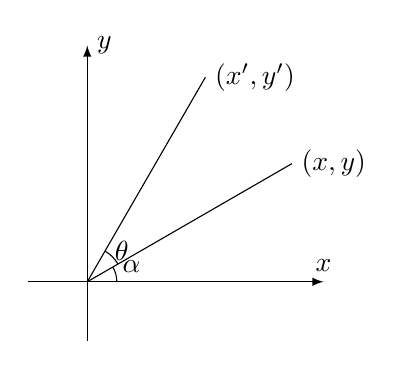
\begin{tikzpicture}[>=latex,scale=.75]
		\draw[->] (-1,0)--(4,0)node[above]{$x$};
		\draw[->] (0,-1)--(0,4)node[right]{$y$};
		\draw[] (0,0)--(30:4)node[right]{$(x,y)$};
		\draw[] (0,0)--(60:4)node[right]{$(x',y')$};
		\draw[] (0:.5) arc (0:30:.5)node[right]{$\alpha$};
		\draw[] (30:.6) arc (30:60:.6)node[right]{$\theta$};
	\end{tikzpicture}
\end{figure}

$$
\begin{aligned}
x'&=r\cos(\theta+\alpha)\\&=r\cos\theta\cos\alpha-r\sin\theta\sin\alpha\\&=x\cos\theta-y\sin\alpha\\
y'&=r\sin(\theta+\alpha)\\&=r\sin\theta\cos\alpha+r\sin\alpha\cos\theta\\&=x\sin\theta+y\cos\theta\\
\end{aligned}
$$

\subsubsection{矩阵的转置}

\index{矩阵转置}

把一个矩阵行列互换,则称处理后的矩阵叫做\textcolor{red}{矩阵的转置},对于矩阵$A$而言:

$$
\begin{pmatrix}
	a_{11} &a_{12}&\cdots&a_{1n}\\
	a_{21}&a_{22}&\cdots&a_{2n}\\
	\vdots&\vdots&\ddots&\vdots\\
	a_{m1}&a_{m2}&\cdots&a_{mn}\\
\end{pmatrix}
$$

矩阵A的转置如下所示:

$$
\begin{pmatrix}
	a_{11} &a_{21}&\cdots&a_{m1}\\
	a_{12}&a_{22}&\cdots&a_{m2}\\
	\vdots&\vdots&\ddots&\vdots\\
	a_{1n}&a_{2n}&\cdots&a_{mn}\\
\end{pmatrix}
$$

显然有$m\times n$的矩阵,转置后为$n\times m$的矩阵

矩阵转置具有如下性质:

\begin{enumerate}
	\item  $(A^T)^T=A$
	\item $(A^T)+B^T=A^T+B^T$
	\item $k(A^T)=(kA)^T$
	\item $(AB)^T=B^TA^T$
\end{enumerate}

\begin{question}
	$(AB)^T=B^TA^T$
	
	\begin{proof}
		首先证明同型,假设A为$m\times p$,B为$p\times n$型矩阵,则$(AB)T$,$B^TA^T$均为$m\times n$

		然后证明矩阵元相等:

		$$
		\begin{aligned}
			(AB)^T&\rightarrow c_{ji}=\sum_{k=1}^p a_{ik}b_{kj}\\
			B^TA^T&\rightarrow c_{ji}=\sum_{k=1}^p b_{kj}a_{ik}\\
		\end{aligned}
		$$

		显然有矩阵元相等
	\end{proof}
\end{question}

若$A^T=A$,则称A为\textcolor{red}{对称矩阵},若$A^T=-A$,则称A为\textcolor{red}{反称矩阵}\index{矩阵!对称矩阵}\index{矩阵!反称矩阵}

显然对称矩阵和反称矩阵都是方阵,且对称矩阵中$a_{ij}=a_{ji},\forall  i,j$

反称矩阵中$a_{ii}=0,a_{ij}=-a_{ji},i\neq j$

对称矩阵的线性运算仍为对称矩阵吗,对称矩阵的乘积不一定为对称矩阵

\begin{question}
	假设A与B都是n阶对称矩阵,证明矩阵AB为对称矩阵的充要条件是AB=BA

	\begin{proof}
		先证充分性:AB=BA,$(AB)^T=B^TA^T=BA$,符合对称矩阵的定义,则AB为对称矩阵

		再证必要性:AB为对称矩阵,$(AB)T=B^TA^T=BA=AB$,所以能够证明AB=BA
	\end{proof}

	\textcolor{red}{对于任意矩阵A,$AA^T$和$A^TA$为对称矩阵}

\end{question}